\documentclass{article}
\usepackage[utf8]{inputenc}

\usepackage{natbib}
\usepackage{graphicx}
\usepackage{amsmath}
\usepackage{amsfonts}
\usepackage{amssymb}
\usepackage{mathtools}
\usepackage{fullpage}
\usepackage{enumitem}
\usepackage{float}
\usepackage{hyperref}
\hypersetup{
    colorlinks=true,
    allcolors=,  % Nothing change colors
    urlcolor=blue  % URL change color
}

\graphicspath{{../images/}}

\title{Problem set 1\\
    \large{Machine Learning}}
\author{Lucas Emanuel Resck Domingues\\    
    Professor: Rodrigo Targino\\\\
    {School of Applied Mathematics}\\
    {Getulio Vargas Foundation}}
\date{\today}

\begin{document}

    \maketitle

    \noindent \textbf{\textit{Exercise 1.3}}

    \noindent \textit{The weight update rule in (1.3)~\cite{yaser2012learning} has the nice interpretation that it moves in the direction of classifying $\mathbf{x}(t)$ correctly.}
    \begin{itemize}[before=\itshape]
        \item[(a)] Show that $y(t) \mathbf{w}^\intercal(t) \mathbf{x}(t) < 0$. [Hint: $\mathbf{x}(t)$ is misclassified by $\mathbf{w}(t)$.]
        \item[(b)] Show that $y(t) \mathbf{w}^\intercal(t + 1) \mathbf{x}(t) > y(t) \mathbf{w}^\intercal(t) \mathbf{x}(t)$. [Hint: Use (1.3)~\cite{yaser2012learning}.]
        \item[(c)] As far as classifying $\mathbf{x(t)}$ is concerned, argue that the move from $\mathbf{w}(t)$ to $\mathbf{w}(t + 1)$ is a move `in the right direction'.
    \end{itemize}

    \begin{itemize}
        \item[(a)] Because $\mathbf{x}(t)$ is misclassified, $\mathbf{w}^\intercal(t) \mathbf{x}(t)$ has the opposite sign of $y(t)$.
        \item[(b)] Note that, because $x_0 = 1$, we have $\mathbf{x}(t) \ne 0$.
            So:
            \begin{align*}
                y(t) \mathbf{w}^\intercal(t + 1) \mathbf{x}(t) &= y(t) (\mathbf{w}(t) + y(t) \mathbf{x}(t))^\intercal \mathbf{x}(t) \\
                &= y(t) (\mathbf{w}^\intercal(t) + y(t) \mathbf{x}^\intercal(t)) \mathbf{x}(t) \\
                &= y(t) \mathbf{w}^\intercal(t) \mathbf{x}(t) + [y(t)]^2 \mathbf{x}^\intercal(t) \mathbf{x}(t)  \\
                &= y(t) \mathbf{w}^\intercal(t) \mathbf{x}(t) + [y(t) \lVert\mathbf{x}\lVert]^2 \\
                &> y(t) \mathbf{w}^\intercal(t) \mathbf{x}(t)
            \end{align*}
        \item[(c)] We would like to have $y(t) \mathbf{w}^\intercal(t) \mathbf{x}(t) > 0$, if the classification of $\mathbf{x}(t)$ was correct.
            So we take a greater $y(t) \mathbf{w}^\intercal(t + 1) \mathbf{x}(t)$, with the hope that it will be positive.
            If it is not the case, we can try again. \\
    \end{itemize}

    \noindent \textbf{\textit{Exercise 1.4}}

    \noindent \textit{Let us create our own target function $f$ and data set $\cal{D}$ and see how the perceptron learning algorithm works.
    Take $d = 2$ so you can visualize the problem, and choose a random line in the plane as your target function, where one side of the line maps to $+1$ and the other maps to $-1$.
    Choose the inputs $\mathbf{x}_n$ of the data set as random points in the plane, and evaluate the target function on each $\mathbf{x}_n$ to get the corresponding output $\mathbf{y}_n$.}

    \noindent\textit{Now, generate a data set of size $20$. Try the perceptron learning algorithm on your data set and see how long it takes to converge and how well the final hypothesis $g$ matches your target $f$.
    You can find other ways to play with this experiment in Problem 1.4.} \\

    The code for this experiment can be found in \href{https://github.com/lucasresck/machine-learning/blob/main/notebooks/exercise_1.4.ipynb}{GitHub}.

    We choose a random line in the plane, as it can be seen in the Figure \ref{fig:random_line}.
    
    \begin{figure}[H]
        \centering
        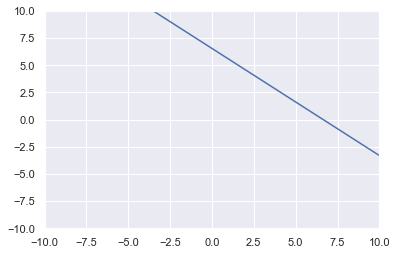
\includegraphics[width=0.6\textwidth]{exercise_1.4_1.png}
        \caption{Random line in the plane.}
        \label{fig:random_line}
    \end{figure}

    We generate a data set of $n = 20$ random points in the plane, and we evaluate the target function, as shown in Figure \ref{fig:data_set}.
    Note that the target function evaluation, in the Figure, is the color of the points.
    
    \begin{figure}[H]
        \centering
        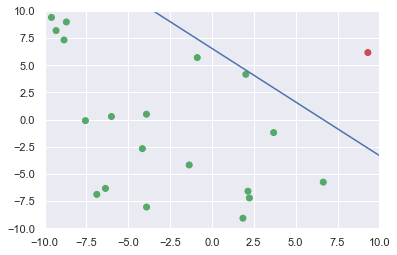
\includegraphics[width=0.6\textwidth]{exercise_1.4_2.png}
        \caption{Random data set and random line in the plane.}
        \label{fig:data_set}
    \end{figure}

    Now we run the perceptron learning algorithm, with 23 iterations, and the result is shown in Figure \ref{fig:pla}.
    We see that, even though the result is the same, the two lines are different.
    
    \begin{figure}[H]
        \centering
        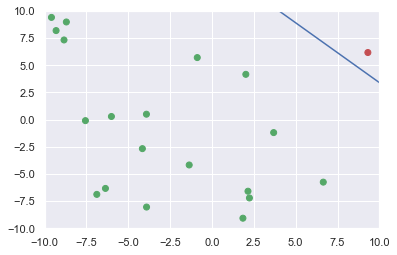
\includegraphics[width=0.6\textwidth]{exercise_1.4_3.png}
        \caption{Line result of perceptron learning algorithm.}
        \label{fig:pla}
    \end{figure}

    \nocite{yaser2012learning}
    \bibliographystyle{plain}
    \bibliography{references}

\end{document}